
\documentclass[fleqn]{beamer}
\usetheme{Madrid}
\usecolortheme{whale}
\usepackage{bm}
\usepackage{graphicx}
\usepackage{subcaption}

\usepackage{tikz}  %TikZ central library is called.
\usepackage{tcolorbox}
\usetikzlibrary{automata,positioning} % automata and positioning libraries are required to use nodes and coordinates in addition to placement propetries.

\title{Elements of collision theory at low energies}
\author{Pan\u{a} Gabriel Tiberiu}
\date{22.07.2019}

 


\newcommand{\vpr}[1]{\vec {p^{\prime}_{#1}}}
\newcommand{\bdm}{\begin{displaymath}}
\newcommand{\edm}{\end{displaymath}}
%\newcommand{\psc}[2]{#1 \cdot #2}
\newcommand{\beq}{\begin{equation}}
\newcommand{\eeq}{\end{equation}}
\newcommand{\beqa}{\begin{eqnarray}}
\newcommand{\eeqa}{\end{eqnarray}}
\newcommand{\hi}{\^{\i}}
\newcommand{\Sch}{Schr\"odinger }
\newcommand{\Schv}{Schr\"odinger}
\newcommand{\tc}{\textcolor}
\newcommand{\edo}{\end{document}}
\newcommand{\npb}{\nopagebreak}
\newcommand{\ssk}{\smallskip}
\newcommand{\msk}{\medskip}
\newcommand{\bsk}{\bigskip}
\newcommand{\mbx}{\mbox{\tiny x}}
\newcommand{\ds}{\displaystyle}
\newcommand{\vs}{\vspace{0.1cm}}
\newcommand{\np}{\newpage}
\newcommand{\bit}{\begin{itemize}}
\newcommand{\eit}{\end{itemize}}
\newcommand{\ben}{\begin{enumerate}}
\newcommand{\een}{\end{enumerate}}
\newcommand{\vem}{\vspace{1em}}
\newcommand{\hem}{\hspace{1em}}
\newcommand{\noi}{\noindent}
\newcommand{\rar}{\rightarrow}
\newcommand{\bfP}{{\bm P}}
\newcommand{\bfp}{{\bm p}}
\newcommand{\bfA}{{\bm A}}
\newcommand{\bfB}{{\bm B}}
\newcommand{\bfC}{{\bm C}}
\newcommand{\balpha}{{\boldsymbol \alpha}}
\newcommand{\bfE}{{\bm E}}
\newcommand{\bfe}{{\bm e}}
\newcommand{\bfF}{{\bm F}}
\newcommand{\bfd}{{\bm d}}
\newcommand{\bfn}{{\bm n}}
\newcommand{\bfkp}{{\boldsymbol \kappa}}
\newcommand{\bfr}{{\bm r}}
\newcommand{\bfAr}{{\bm A}(\bfr)}
\newcommand{\hbr}{\hat{\bm r}}
\newcommand{\bfJ}{{\bm J}}
\newcommand{\bfS}{{\bm S}}
\newcommand{\bfs}{{\bm s}}
\newcommand{\bfk}{{\bm k}}
\newcommand{\hbp}{{\hat{\bm p}}}
\newcommand{\hbk}{\hat{\bm k}}
\newcommand{\bfq}{{\bm q}}
\newcommand{\bfV}{{\bm V}}
\newcommand{\bfv}{{\bm v}}
\newcommand{\bfsg}{{\bm \sigma}}
\newcommand{\bnabla}{{\boldsymbol \nabla}}
\newcommand{\slm}{\sum_{l=0}^{\infty}\sum_{m=-l}^{l}}
\newcommand{\slmp}{\sum_{l'=0}^{\infty}\sum_{m'=-l'}^{l'}}
\newcommand{\viq}{\, , \qquad}
\newcommand{\ra}{\rangle}
\newcommand{\la}{\langle}
\newcommand{\tg}{\mathrm{\,tg\,}}
\newcommand{\cotg}{\mathrm{\,cotg\,}}
\newcommand{\arctg}{\mathrm{\,arctg\,}}
\newcommand{\ai}{{\^{\i}}}






%%% Local Variables:
%%% mode: latex
%%% TeX-master: "main"
%%% End:

\begin{document}
\footnotesize
  \maketitle
  \begin{frame}[allowframebreaks]{Contents}
   \tableofcontents
  \end{frame}

  \section{Introduction}
\begin{frame}{Introduction}
Importance of low energy collisions\\
\begin{itemize}
  \item study of gas cooling methods such as:\\
  - evaporation in magnetic traps;\\
  - optic manipulation using lasers.
  \item ultra-cold gases can be used for:\\
  - precision measuring of atomic and molecular parameters;\\
  - study of wave-matter coherences which occur at low enegies;\\
  - statistics of quantum condensates formed by weak interacting atoms.
\end{itemize}

Goal of this paper:\\
We demonstrate that collisions at low energies can be defined by a single parameter: the scattering lenght. We will analyze the theoretical model which helps us calculate this parameter and we will look at a few simple potentials and determine their scattering lenghts. 
\end{frame}

\section{Elements of collision theory}

\subsection{The scattering cross section}

\begin{frame}{Collisions in classical mechanics}
In a scattering experiment, we observe collisions between a flux of incident particles and a target material.\\~\\

The differential cross section:
\begin{align}
\frac{d\sigma(\theta,\varphi)}{d\Omega}=\frac{1}{J_{inc}}\frac{dN(\theta,\varphi)}{d\Omega} 
\end{align}
\\~\\
$\sigma$ represents the total cross section: 
\begin{align}
\sigma=\int\frac{d\sigma}{d\Omega}d\Omega=\int_{0}^{\pi}\sin\theta d\theta\int_{0}^{2\pi}\frac{d\sigma(\theta,\varphi)}{d\Omega}d\varphi
\end{align} 
\end{frame}

\begin{frame}{Collisions in classical mechanics: Lab and CM frames}
\begin{figure}[h]
\centering

\begin{subfigure}{.5\textwidth}
  \centering
\begin{tcolorbox}[colback=white]
 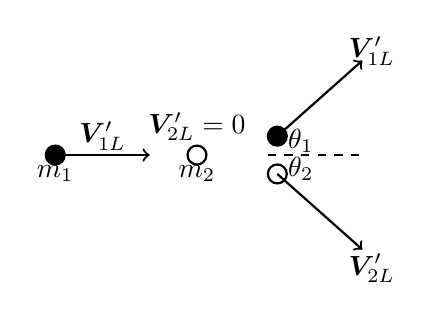
\begin{tikzpicture}[thick, scale=0.6]
\draw [thick, ->] (4.5,4) -- (6.5,4);
\draw [thick, ->] (9.2,4.4) -- (11,6);
\draw [thick, ->] (9.2,3.6) -- (11,2);
\draw [ dashed] (9,4) -- (11,4);
\node at (4.5,3.6) {$m_1$};
\node at (7.5,3.6) {$m_2$};
\node at (9.7,4.3) {$\theta_1$};
\node at (9.7,3.7) {$\theta_2$};
\node at (5.5,4.4) {${\bm V}'_{1L}$};
\node at (7.5,4.6) {${\bm V}'_{2L}=0$};
\node at (11.2,6.2) {${\bm V}'_{1L} $};
\node at (11.2,1.6) {${\bm V}'_{2L} $};
\draw [fill] (4.5,4) circle [radius=0.2];c
\draw (7.5,4) circle [radius=0.2];c
\draw [fill] (9.2,4.4) circle [radius=0.2];c
\draw  (9.2,3.6) circle [radius=0.2];c
\end{tikzpicture}
\end{tcolorbox}
  \caption{Lab frame}
  \label{fig:sub21}
\end{subfigure}%
\begin{subfigure}{.5\textwidth}
  \centering
  \begin{tcolorbox}[colback=white]
  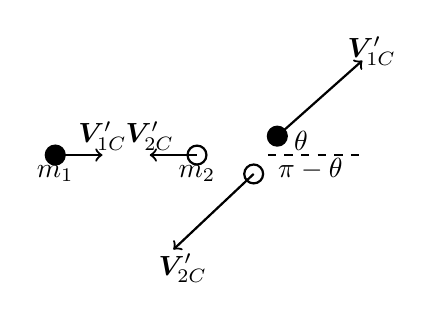
\begin{tikzpicture}[thick, scale=0.6]
\draw [thick, ->] (4.5,4) -- (5.5,4);
\draw [thick, ->] (7.5,4) -- (6.5,4);
\draw [thick, ->] (9.2,4.4) -- (11,6);
\draw [thick, ->] (8.7,3.6) -- (7,2);
\draw [ dashed] (9,4) -- (11,4);
\node at (4.5,3.6) {$m_1$};
\node at (7.5,3.6) {$m_2$};
\node at (9.7,4.3) {$\theta$};
\node at (9.9,3.7) {$\pi-\theta$};
\node at (5.5,4.4) {${\bm V}'_{1C} $};
\node at (6.5,4.4) {${\bm V}'_{2C} $};
\node at (11.2,6.2) {${\bm V}'_{1C}$};
\node at (7.2,1.6) {${\bm V}'_{2C}$};
\draw [fill] (4.5,4) circle [radius=0.2];c
\draw (7.5,4) circle [radius=0.2];c
\draw [fill] (9.2,4.4) circle [radius=0.2];c
\draw  (8.7,3.6) circle [radius=0.2];c
\end{tikzpicture}
\end{tcolorbox}
  \caption{Center of Mass frame}
  \label{fig:sub22}
\end{subfigure}
\caption{Elastic scattering of two point-like particles in Lab and CM frames: a particle of mass $m_1$ collides with a particle $m_2$ which is at rest}
\label{fig:ciocniri}
\end{figure}

\end{frame}

\begin{frame}{Lab and CM frames}
The relation between cross sections in Lab and CM frames:
\begin{align}
\left(\frac{d\sigma}{d\Omega_1}\right)_{SL}=\frac{(1+\frac{m^2_1}{m^2_2}+2\frac{m_1}{m_2}\cos\theta)^{3/2}}{1+\frac{m_1}{m_2}\cos\theta}\left(\frac{d\sigma}{d\Omega}\right)_{SCM}
\end{align}
\\
Limiting cases:\\
a) $m_2\gg m_1$ sau $\frac{m_1}{m_2} \xrightarrow{}0$ results in Lab and CM are identical $\left(\frac{d\sigma}{d\Omega_1}\right)_{SL}=\left(\frac{d\sigma}{d\Omega}\right)_{SCM}$ deoarece $\theta_1=\theta$\\
b) $m_2=m_1$ then $\tan\theta_1=\tan\frac{\theta}{2}$ or $\theta_1=\frac{\theta}{2}$ resulting in
\begin{align}
\boxed{\left(\frac{d\sigma}{d\Omega_1}\right)_{SL}=4\left(\frac{d\sigma}{d\Omega}\right)_{SCM}\cos\frac{\theta}{2}}
\end{align}

\end{frame} 


\subsection{The Schr\"{o}dinger equation}
\begin{frame}{Collisions in quantum mechanics}
\begin{figure}[h]
\centering
\begin{tcolorbox}[colback=white]
 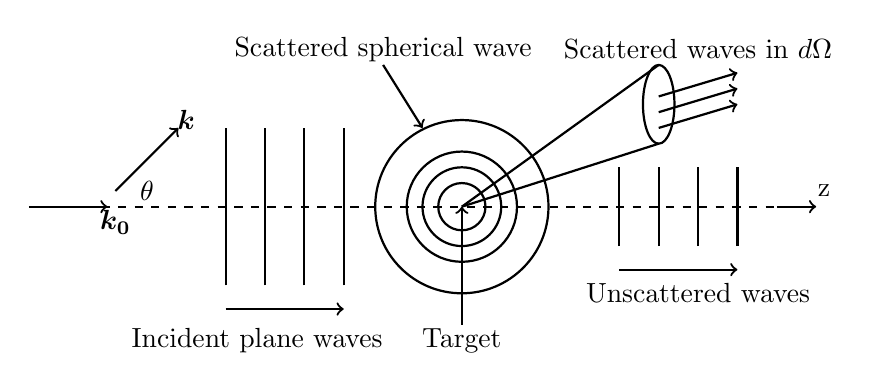
\begin{tikzpicture}[thick, scale=1]
\draw [dashed] (2,4) -- (11,4);

\draw [thick, ->] (1.5,4) -- (2.5,4);
\node at (2.6,3.8) {$\bm{k_0}$};
\draw [thick, ->] (2.6,4.2) -- (3.4,5);
\node at (3.5,5.1) {$\bm{k}$};
\node at (3,4.2) {$\theta$};
\draw [thick, ->] (11,4) -- (11.5,4);
\node at (11.6,4.2) {z};

\draw [thick, -] (4,3) -- (4,5);
\draw [thick, -] (4.5,3) -- (4.5,5);
\draw [thick, -] (5,3) -- (5,5);
\draw [thick, -] (5.5,3) -- (5.5,5);
\draw [thick, ->] (4,2.7) -- (5.5,2.7);
\node at (4.4,2.3) {Incident plane waves};

\draw (7,4) circle [radius=0.3];c
\draw (7,4) circle [radius=0.5];c
\draw (7,4) circle [radius=0.7];c
\draw (7,4) circle [radius=1.1];c
\draw [thick, ->] (6,5.8) -- (6.5,5);
\node at (6,6) {Scattered spherical wave}; 
\draw [thick, ->] (7,2.5) -- (7,4);
\node at (7,2.3) {Target};

\draw [thick, -] (7,4) -- (9.5,5.8);
\draw [thick, -] (7,4) -- (9.5,4.8);
\node at (10,6) {Scattered waves in $d\Omega$};
\draw (9.5,5.3) ellipse (0.2 and 0.5);
\draw [thick, ->] (9.5,5.0) -- (10.5,5.3);
\draw [thick, ->] (9.5,5.2) -- (10.5,5.5);
\draw [thick, ->] (9.5,5.4) -- (10.5,5.7);

\draw [thick, -] (9,3.5) -- (9,4.5);
\draw [thick, -] (9.5,3.5) -- (9.5,4.5);
\draw [thick, -] (10,3.5) -- (10,4.5);
\draw [thick, -] (10.5,3.5) -- (10.5,4.5);
\draw [thick, ->] (9,3.2) -- (10.5,3.2);
\node at (10,2.9) {Unscattered waves};
\end{tikzpicture}
\end{tcolorbox}
  \caption{Scattering of plane waves on a central potential}
  \label{fig:collision quantum mec}
\end{figure}
\end{frame}

\begin{frame}{Schr\"{o}dinger equation}
The scattering problem of two non-relativistic, spinless particles with masses $m_1,m_2$ becomes the scattering of a particle of mean mass $\mu$ defined by a plane wave on a central potential.\\
Schr\"{o}dinger equation:
\begin{align}
-\frac{\hbar^2}{2\mu}\nabla^2\psi({\bm r})+V({\bm r})\psi({\bm r})=E\psi({\bm r})
\end{align}
We assume the potential has finite range.\\
The wave function which describes the scattering is a superposition of the incident plane wave and the scattered, outgoing spherical wave:
\begin{align}
&\psi({\bm r})=\phi_{inc}({\bm r})+\phi_{sc}({\bm r})
\end{align}
\end{frame} 

\begin{frame}{The Schr\"{o}dinger equation solution}
\begin{figure}[h]
\centering
\begin{tcolorbox}[colback=white]
 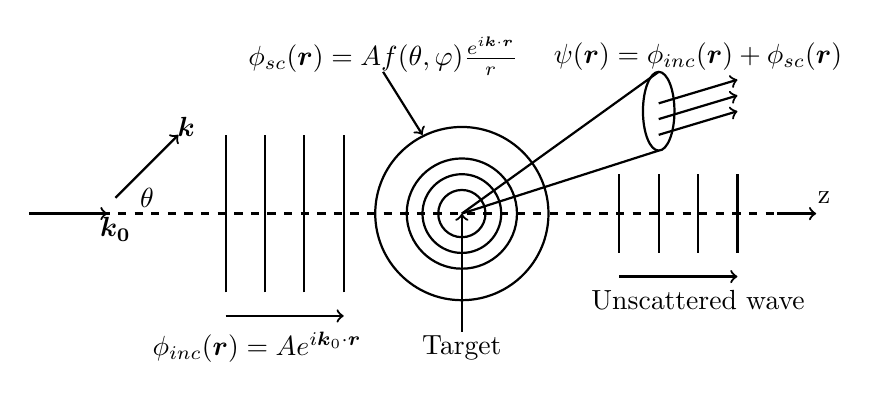
\begin{tikzpicture}[thick, scale=1]
\draw [dashed] (2,4) -- (11,4);

\draw [thick, ->] (1.5,4) -- (2.5,4);
\node at (2.6,3.8) {$\bm{k_0}$};
\draw [thick, ->] (2.6,4.2) -- (3.4,5);
\node at (3.5,5.1) {$\bm{k}$};
\node at (3,4.2) {$\theta$};
\draw [thick, ->] (11,4) -- (11.5,4);
\node at (11.6,4.2) {z};

\draw [thick, -] (4,3) -- (4,5);
\draw [thick, -] (4.5,3) -- (4.5,5);
\draw [thick, -] (5,3) -- (5,5);
\draw [thick, -] (5.5,3) -- (5.5,5);
\draw [thick, ->] (4,2.7) -- (5.5,2.7);
\node at (4.4,2.3) {$\phi_{inc}({\bm r})=Ae^{i{\bm k_0}\cdot{\bm r}}$};

\draw (7,4) circle [radius=0.3];c
\draw (7,4) circle [radius=0.5];c
\draw (7,4) circle [radius=0.7];c
\draw (7,4) circle [radius=1.1];c
\draw [thick, ->] (6,5.8) -- (6.5,5);
\node at (6,6) {$\phi_{sc}({\bm r})=A f(\theta,\varphi)\frac{e^{i{\bm k}\cdot{\bm r}}}{r}$}; 
\draw [thick, ->] (7,2.5) -- (7,4);
\node at (7,2.3) {Target};

\draw [thick, -] (7,4) -- (9.5,5.8);
\draw [thick, -] (7,4) -- (9.5,4.8);
\node at (10,6) {$\psi({\bm r})=\phi_{inc}({\bm r})+\phi_{sc}({\bm r})$};
\draw (9.5,5.3) ellipse (0.2 and 0.5);
\draw [thick, ->] (9.5,5.0) -- (10.5,5.3);
\draw [thick, ->] (9.5,5.2) -- (10.5,5.5);
\draw [thick, ->] (9.5,5.4) -- (10.5,5.7);

\draw [thick, -] (9,3.5) -- (9,4.5);
\draw [thick, -] (9.5,3.5) -- (9.5,4.5);
\draw [thick, -] (10,3.5) -- (10,4.5);
\draw [thick, -] (10.5,3.5) -- (10.5,4.5);
\draw [thick, ->] (9,3.2) -- (10.5,3.2);
\node at (10,2.9) {Unscattered wave};
\end{tikzpicture}
\end{tcolorbox}
  \label{fig:general solution}
\end{figure}
\begin{align}
\psi({\bm r})=A \left[ e^{i{\bm k_0}\cdot{\bm r}}+f(\theta,\varphi)\frac{e^{i{\bm k}\cdot{\bm r}}}{r}\right] \quad \textbf{, $f(\theta,\varphi)=$ the scattering amplitude}
\end{align}

\end{frame}

\begin{frame}{The scattering amplitude}
We now look for the connection between the scattering amplitude and the differential cross section.
We introduce the flux densities:
\begin{align}
&J_{inc}=|A|^2 \frac{\hbar k_0}{\mu}\\
&J_{sc}=|A|^2 \frac{\hbar k}{\mu r^2}|f(\theta,\varphi)|^2=\frac{k}{k_0}\frac{J_{inc}}{r^2}|f(\theta,\varphi)|^2
\end{align}
Number of scattered particles:
\begin{align}
dN(\theta,\varphi)=J_{sc}r^2d\Omega
\end{align}
Using this result and the definition of the differential cross section we find:
\begin{align}
\frac{d\sigma}{d\Omega}=\frac{1}{J_{inc}}\frac{dN}{d\Omega}=\frac{1}{J_{inc}}J_{sc}r^2=\frac{k}{k_0}|f(\theta,\varphi)|^2
\end{align}
In the case of ellastic scattering $k=k_0$, so we obtain:
\begin{align}
\frac{d\sigma}{d\Omega}=|f(\theta,\varphi)|^2
\end{align}

\end{frame} 

\subsection{Partial wave analysis. Phase shifts.}
\begin{frame}{Partial wave analysis}
We assume the potential has spherical symmetry. The angular momentum of the particle is conserved after scattering so we can define the incident plane wave as a superposition of angular momentum eigenstates, each described by a quantum number $l$: 
\begin{align}
e^{i{\bm k}\cdot{\bm r}}=e^{ikr\cos\theta}=\sum_{l=0}^{\infty}i^l(2l+1)j_l(kr)P_l(\cos\theta) 
\end{align}
where $j_l$ are the spherical Bessel functions. We recall:
\begin{align}
\psi({\bm r})=A \left[ e^{i{\bm k_0}\cdot{\bm r}}+f(\theta,\varphi)\frac{e^{i{\bm k}\cdot{\bm r}}}{r}\right]
\end{align}
Using the two results (witch $\varphi=0$):
\begin{align}
\psi(r,\theta)\simeq\sum_{l=0}^{\infty}i^l(2l+1)j_l(kr)P_l(\cos\theta)+f(\theta)\frac{e^{ikr}}{r}
\end{align}
Also, the general solution of the Scr\"{o}dinger equation for a spherically symmetric potential is:
\begin{align}
\psi(r,\theta)=\sum_{l=0}^{\infty}a_lR_{kl}(r)P_l(\cos\theta) 
\end{align}
\end{frame} 

\begin{frame}[allowframebreaks]{Asymptotic form}
The radial equation:
\begin{align}
\left[\frac{d^2}{dr^2}+k^2-\frac{l(l+1)}{r^2}\right](rR_{kl}(r))=\frac{2m}{\hbar^2}V(r)(rR_{kl}(r))
\end{align}
For $r\to\infty \Rightarrow V\to0$, the equation becomes:
\begin{align}
\left(\frac{d^2}{dr^2}+k^2\right)(rR_{kl}(r))=0 \label{ecrad2}
\end{align}
The general solution of this equation can be written in term of Bessel and Neumann functions:
\begin{align}
R_{kl}(r)=A_lj_l(kr)+B_ln_l(kr)
\end{align}
with asymptotic behavior:
\begin{align}
R_{kl}(r) \to A_l \frac{\sin(kr-l\pi/2)}{kr}-B_l\frac{\cos(kr-l\pi/2)}{kr}
\end{align}
If $V=0$ for any $r$ (free particle), the solution for equation (\ref{ecrad2}) must be zero for $r=0$. The Neumann function diverges at $r=0$, so we must cut out the cosine term.\\
We re-write the sollution:
\begin{align}
R_{kl}(r)\to C_l\frac{sin(kr-l\pi/2+\delta_l)}{kr}
\end{align}
where $A_l=C_l\cos\delta_l$ and $B_l=-C_l\sin\delta_l$, so $C_l=\sqrt{A^2_l+B^2_l}$ and
\begin{align}
\boxed{tan\delta_l=-\frac{B_l}{A_l}} \Rightarrow \delta_l=-\tan^{-1}\left(\frac{B_l}{A_l}\right)
\end{align}
{\bf where $\delta_l$ is called the phase shift}.
\end{frame} 

\begin{frame}[allowframebreaks]{The phase shift. Connection with the differential cross section}

\begin{align}
&R_{kl}(r)\to C_l\frac{sin(kr-l\pi/2+\delta_l)}{kr}\\
&\delta_l=0 \Rightarrow  R_{kl}(r)\to C_l\frac{sin(kr-l\pi/2)}{kr} \to C_l j_l(kr)
\end{align}
{\bf The phase shift $\delta_l$ is a real angle which vanishes for any value of $l$ in absence of a potential $V=0$. It measures, at large values of $r$ the degree to which $R_{kl}$ differs from $j_l(kr)$.\\
Because the phase shift appears due to the potential acting upon the particle, we expect that the differential cross section will depend on $\delta_l$.} 
\\~\\
Using the asympotic form obtained for $R_kl(r)$, we find the asymptotic form for $\psi(r,\theta)$:
\begin{align}
\psi(r,\theta)\to\sum_{l=0}^{\infty}a_lP_l(\cos\theta)\frac{\sin(kr-l\pi/2+\delta_l)}{kr},(r\to\infty)
\end{align}
The previous equation is called the distorted plane waves (due to the phase shift) and can be written:
\begin{align}
\boxed{\psi(r,\theta)\to -\frac{e^{-ikr}}{2ikr}\sum_{l=0}^{\infty}a_li^le^{-i\delta_l}P_l(\cos\theta)+\frac{e^{ikr}}{2ikr}\sum_{l=0}^{\infty}a_l(-i)^le^{i\delta_l}P_l(\cos\theta)} \label{ecuatie276}
\end{align}
We recall:
\begin{align}
\psi(r,\theta)\simeq\sum_{l=0}^{\infty}i^l(2l+1)j_l(kr)P_l(\cos\theta)+f(\theta)\frac{e^{ikr}}{r}
\end{align}
Which can be written:
\begin{align}
\hspace*{-1cm}\boxed{\psi(r,\theta)\to-\frac{e^{-ikr}}{2ikr}\sum_{l=0}^{\infty}i^{2l}(2l+1)P_l(\cos\theta)+\frac{e^{ikr}}{r}\left[f(\theta)+\frac{1}{2ik}\sum_{l=0}^{\infty}i^l(-i)^l(2l+1)P_l(\cos\theta)\right]} \label{ecuatie268}
\end{align}
Equating the coefficients of $e^{ikr}/r$ and $e^{-ikr}/r$ we obtain the scattering amplitude:
\begin{align}
&f(\theta)=\frac{1}{k}\sum_{l=0}^{\infty}(2l+1)e^{i\delta_l}\sin\delta_lP_l(\cos\theta)\\
&\frac{d\sigma}{d\Omega}=|f(\theta)|^2=\frac{1}{k^2}\sum_{l=0}^{\infty}\sum_{l'=0}^{\infty}(2l+1)
(2l'+1)e^{i(\delta_l-\delta_{l'})}\sin\delta_l\sin\delta_{l'}P_l(\cos\theta)P_{l'}(\cos\theta),\\
&\boxed{\sigma=\sum_{l=0}^{\infty}\sigma_l=\frac{4\pi}{k^2}\sum_{l=0}^{\infty}(2l+1)\sin^2\delta_l}
\end{align}

\end{frame} 

\subsection{Low energies limit. The scattering length}
\begin{frame}{Low energies limit. The scattering length}
For any other partial wave rather than $l=0$ the interatomic potential in the Schr\"{o}dinger equation is overlapped by the centrifugal barrier $\hbar^2l(l+1)/2\mu r^2$. At low energies, this barrier dominates the potential, particles would be scattered by this barrier. So we can talk in terms of scattering at low energies on the potential $V(r)$ only for $l=0$ (s-wave scattering).\\
For $E\to0$ and large $r$ so that $V(r)=0$, the radial equation becomes:
\begin{align}
\frac{d^2R}{dr^2}=0, \quad \text {with straight line solution:}\quad R(r)=C(r-a)
\end{align}
This is the $k\to 0$ limit of 
\begin{align}
R(r)=C'\sin(kr+\delta_0(k)),\quad \text{ which means}\quad \delta_0(k)=-ka 
\end{align}
{\bf The quantity $a$ is called the scattering lenght and it represents the point where the extrapolated external wavefunction intersects the axis.}\\
We write the differential cross section for low energy:
\begin{align}
\lim_{k\to 0}\sigma_{l=0}(k)=4\pi a^2
\end{align}
\end{frame} 

\begin{frame}{Recap}
Differential cross section:
\begin{align}
\frac{d\sigma(\theta,\varphi)}{d\Omega}=\frac{1}{J_{inc}}\frac{dN(\theta,\varphi)}{d\Omega} 
\end{align}
Scattering amplitude:
\begin{align}
\psi({\bm r})=A \left[ e^{i{\bm k_0}\cdot{\bm r}}+f(\theta,\varphi)\frac{e^{i{\bm k}\cdot{\bm r}}}{r}\right],  \qquad  \boxed{\frac{d\sigma}{d\Omega}=|f(\theta,\varphi)|^2}
\end{align}
Phase shift:
\begin{align}
R_{kl}(r)\to C_l\frac{sin(kr-l\pi/2+\delta_l)}{kr}, \qquad  \boxed{tan\delta_l=-\frac{B_l}{A_l}}
\end{align}
Cross section using phase shift:
\begin{align}
\boxed{\sigma=\sum_{l=0}^{\infty}\sigma_l=\frac{4\pi}{k^2}\sum_{l=0}^{\infty}(2l+1)\sin^2\delta_l}
\end{align}
Scattering length:
\begin{align}
\boxed{a=-\lim_{k\to 0}\frac{\tan\delta_0(k)}{k}}
\end{align}
%&f(\theta)=\frac{1}{k}\sum_{l=0}^{\infty}(2l+1)e^{i\delta_l}\sin\delta_lP_l(\cos\theta)\\
\end{frame}

\section{Numerical results}

\subsection{Scattering lenght for some simple potentials}
\begin{frame}[allowframebreaks]{Algorithm}
We write the radial Schr\"{o}dinger equation:
\begin{align}
&\chi''({\bm r})+(\frac{2M}{\hbar^2}(E({\bm k})-V({\bm r}))-\frac{l(l+1)}{r^2})\chi({\bm r})=0 \label{srad}
\end{align}
for $l=0$, we will integrate it using the starting conditions:
\begin{align}
 &\chi(\epsilon)=\epsilon^{l+1},\quad \chi'(\epsilon)=(l+1)\epsilon^l
\end{align}
on the interval $r\in (\epsilon,r_{Max})$, where $\epsilon$ is chosen very small and $r_{Max}$ is smaller than the range of the potential.\\
For $r>r_{Max}$ the solution can be written as a combination of spherical Bessel functions:
 \begin{align}
&\chi(r_{Max})=A s_l(r_{Max}) +B c_l(r_{Max})\label{eq1}\\
&\chi'(r_{Max})=A s_l'(r_{Max}) +B c_l'(r_{Max})\label{eq2}
\end{align}
where $s_l(r_{Max})=r_{Max}j_0(k r_{Max})$ \c{s}i $c_l(r_{Max})=r_{Max} y_0 (k r_{Max})$
\begin{align}
&\tan \delta_l=-\frac{B}{A}\\
&a=-\lim_{k\to 0}\frac{\tan\delta_0(k)}{k}
\end{align}
\end{frame}

\begin{frame}[allowframebreaks]{Numerov's method for solving differential equations}
We solve the Schr\"{o}dinger equation using the implicit Numerov method.
\begin{align}
&-\frac{\hbar^2}{2M}\frac{d^2u}{dx^2}+V(x)u(x)=Eu(x)\\
&\frac{d^2u}{dx^2}-\frac{2MV(x)}{\hbar^2}u(x)+\frac{2ME}{\hbar^2}u(x)=0\\
&\frac{d^2u}{dx^2}+[k^2-U(x)]u(x)=0
\end{align}
We initialise a grid of steps $N=x_{max}/\epsilon$ and for each step $\epsilon$ we are going to calculate the radial funcion. Using the starting conditions (the first two values of the function) we calculate the rest of the steps.
\begin{align}
&u_1=u(\epsilon)=\epsilon\\
&u_2=u(2\epsilon)=2\epsilon\\
&u_{i+1}=\frac{u_{i-1}\left[1-\frac{\epsilon^2}{12}(U_{i-1}-k^2)\right]-2u_i\left[1+\frac{5\epsilon^2}{12}(U_i-k^2)\right]}{\frac{\epsilon^2}{12}(U_{i+1}-k^2)-1}
\end{align}

\newpage
Once we have the solution we select part of it which is beyond the range of the potential.\\
We fit the solution using a combination of Bessel and Neumann functions, and using its coefficients we calculate the phase shift and scattering length.
\begin{align}
&u(r)=A\sin(kr)+B\cos(kr)\\
&\tan\delta_l=-\frac{B}{A}\\
&a=-\lim_{k\to 0}\frac{\tan\delta_0(k)}{k}
\end{align}
\end{frame}

\begin{frame}[allowframebreaks]{Treapta de poten\c{t}ial}
\begin{align}
V({\bm r})=V(0)\tanh{\frac{{\bm r}-r_0}{\alpha_0}}-V(0)
\end{align}
unde $\alpha_0$ controleaz\u{a} rotunjirea treptei, iar $r_0$ este raza de ac\c{t}iune \c{s}i am ales $M =10^3$ 

\begin{figure}[h!]
\centering
\begin{subfigure}{.5\textwidth}
  \centering
  \includegraphics[width=0.9\linewidth]{PotentialTreapta}
  \caption{Poten\c{t}ial Treapt\u{a}}
  \label{fig:sub311}
\end{subfigure}%
\begin{subfigure}{.5\textwidth}
  \centering
  \includegraphics[width=0.9\linewidth]{LungimeImprastiereTreapta}
  \caption{Lungimea de \^{i}mpr\u{a}\c{s}tiere}
  \label{fig:sub312}
\end{subfigure}
\caption{Treapta de poten\c{t}ial}
\label{fig:treapta}
\end{figure}

\end{frame}

\begin{frame}[allowframebreaks]{Groapa de poten\c{t}ial}
\begin{align}
V({\bm r})=-V(0)\tanh{\frac{{\bm r}-r_0}{\alpha_0}}+V(0)
\end{align}
valorile parametrilor au fost p\u{a}strate
\begin{figure}[h!]
\centering
\begin{subfigure}{.5\textwidth}
  \centering
  \includegraphics[width=0.9\linewidth]{PotentialGroapa}
  \caption{Poten\c{t}ial Groap\u{a}}
  \label{fig:sub321}
\end{subfigure}%
\begin{subfigure}{.5\textwidth}
  \centering
  \includegraphics[width=0.9\linewidth]{LungimeImprastiereGroapa}
  \caption{Lungimea de \^{i}mpr\u{a}\c{s}tiere}
  \label{fig:sub322}
\end{subfigure}
\caption{Groapa de poten\c{t}ial}
\label{fig:groapa}
\end{figure}
\end{frame}

\begin{frame}[allowframebreaks]{Poten\c{t}ial de tip Van der Waals}
\begin{align}
V({\bm r})=V(0)\left(\left(\frac{r_0}{{\bm r}}\right)^12-2\left(\frac{r_0}{{\bm r}}\right)^6\right), \qquad \text{unde } V(0)=10^{-6}
\end{align}

\begin{figure}[h!]
\centering
\begin{subfigure}{.5\textwidth}
  \centering
  \includegraphics[width=0.9\linewidth]{PotentialVanDerWaals}
  \caption{Poten\c{t}ial de tip Van der Waals}
  \label{fig:sub331}
\end{subfigure}%
\begin{subfigure}{.5\textwidth}
  \centering
  \includegraphics[width=0.9\linewidth]{LungimeImprastiereVanDerWaals}
  \caption{Lungimea de \^{i}mpr\u{a}\c{s}tiere}
  \label{fig:sub332}
\end{subfigure}
\caption{Poten\c{t}ial de tip Van der Waals}
\label{fig:groapa}
\end{figure}
\end{frame}

\subsection{Poten\c{t}ial aproximat pentru atomi de Cs.}
\begin{frame}[allowframebreaks]{Poten\c{t}ial aproximat pentru atomi de Cs}
\begin{align}
V(r)=\frac{1}{2}Br^\alpha e^{-\beta r}-\left(\frac{C_6}{r^6}+\frac{C_8}{r^8}+\frac{C_{10}}{r^{10}}\right)f_c(r) \label{vcs}
\end{align}
Primul termen de dup\u{a} egal reprezint\u{a} repulsia dintre electronii de valen\c{t}\u{a}, iar al doilea reprezint\u{a} suma termenilor Van der Waals, \^{i}nmul\c{t}it\u{a} cu o func\c{t}ie de cutoff $f_c(r)$, ce are rolul de a anula divergen\c{t}a $1/r^n$ la distan\c{t}e mici.\\
Func\c{t}ia de cutoff are forma:
\begin{align}
f_c(r)=\Theta(r-r_c)+\Theta(r_c-r)e^{-(rc/r-1)^2},
\end{align}
\begin{center}
 \begin{tabular}{||c c c c c c c||} 
 \hline
 B & $\alpha$ & $\beta$ & $C_6$ & $C_8$ & $C_{10}$ & $r_c$ \\ [0.5ex] 
 \hline 
 0.0016 & 5.53 & 1.072 & 7020 & $1.1 \times 10^6$ & $1.7 \times 10^8$ & 23.165 \\ 
  \hline
\end{tabular}
\end{center}
\newpage
Prezen\c{t}a barierei \^{i}nalte \c{s}i largi face ca la energii mici propagarea solu\c{t}iei ``pe sub barier\u{a}" s\u{a} duc\u{a} la pierderea complet\u{a} a preciziei.
\begin{figure}[h!]
  \centering
  \includegraphics[scale = 0.8]{CS.jpg}
  {\caption{Potentialul (\ref{vcs})\label{gvcs}}}
  \end{figure}
  \^{I}n figur\u{a} este reprezentat\u a solu\c tia $\chi(r)$ g\u asit\u a cu Mathematica pentru $k=0.05$ u.a. Este evident c\u a solu\c tia nu are comportarea corect\u a la distan\c te mari.
\begin{figure}[h!]
  \centering
  \includegraphics[scale = 0.8]{FIG.jpg}
  {\caption{Solu\c{t}ia $\chi(r)$ pentru poten\c{t}ialul (\ref{vcs})\label{figpsi}}}
  \end{figure}
  
\end{frame}

\section{Conclusion}
\begin{frame}[allowframebreaks]{Conclusion}

\begin{itemize}
\item Scattering on simple potentials can be expressed in terms of a single parameter: the scattering lenght.
\item The sign of the scattering lenght can be a good indicative for the ability or failure to obtain a condensate. 
\end{itemize}

\end{frame}

\section{Reference list}
\begin{frame}[allowframebreaks]{Reference list}
\begin{thebibliography}{1000}
\bibitem{art-VW}G. F. Gribakin, V. V. Flambaum, Phys. Rev. A {\bf 48}, 546 (1993).

\bibitem{Zettili}Nouredine Zettili, Quantum Mechanics Concepts and Aplications, 2nd ed

\bibitem{varenna}Jean Dalibard, Collisional dynamics of ultra-cold atomic gases

\bibitem{Szmytk}Radoslaw Szmytkowski, Analytical calculations of scattering lenghths in atomic physics, J. Phys. A: Math. Gen. 28 (1995) 7333-7345
  
\bibitem{IHP-2007}Claude Cohen-Tannoudji. Atom-atom interactions in ultracold gases. DEA. Institut Henri Poincar\`{e}, 25 et 27 Avril 2007, 2007. $<$ cel-00346023 $>$

\bibitem{Jullienne-RMP-ColdCollisions}John Weiner, V. S. Bagnato, S. Zilio, Paul S. Jullienne, Rev. Mod. Phys, Vol 71, No. 1, January 1999

\bibitem{ris}H. Ouerdane, M. Jamieson, D. Vranceanu and M. Cavagnero, J. Phys. B  {\bf 36}, 4075 (2005).
\end{thebibliography}
\end{frame}


%%% Local Variables:
%%% mode: latex
%%% TeX-master: "../main"
%%% End:

  
\end{document}
lexanr
%%% Local Variables:
%%% mode: latex
%%% TeX-master: t
%%% End:
